\section{El Problema de las Distancias Más Cortas}
El problema de las distancias más cortas es uno de los temas más estudiados en la teoría de grafos por sus numerosas aplicaciones, incluyendo la ingeniería de redes, la logística, inteligencia artificial y la investigación operativa. El problema trata sobre un grafo que es una estructura compuesta por nodos y aristas. Cada arista es una conexión entre vértices y puede tener un peso asociado que representa la "distancia" o el "costo" de viajar entre dichos nodos. Se desea hallar la ruta de menor coste entre dos nodos.

\subsection{Ejemplo 1}
\textbf{Algoritmo de Floyd Warshall}
Imaginemos la situación de un repartidor de agua que decide crear una red de entrega de suministros a domicilio con la intención de repartir sus pedidos en el menor tiempo posible. Inicialmente sólo opera únicamente en seis casas, que puedes cubrir gracias a la facilidad de desplazarse entre ellas.
Sin embargo, desea encontrar las rutas más cortas a seguir entre su local y la de sus clientes para cumplir con las entregas de la manera más óptima. Por ello, realizamos el análisis para saber todas las posibles rutas que utilizaría el repartidor.
%%%%%%%%%
\begin{figure}[H]
	\centering
	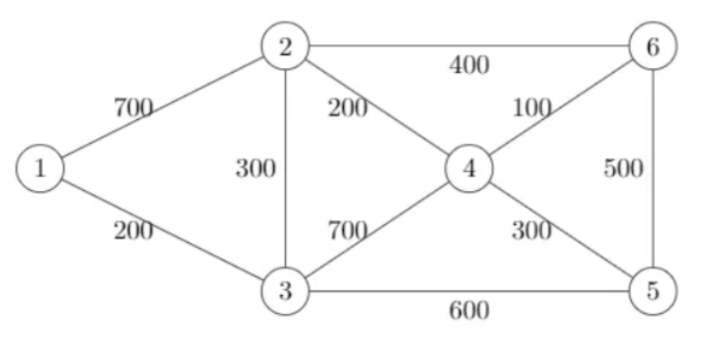
\includegraphics[width=0.8\textwidth]{distancias_cortas_RepresentacionG1.png}
	\caption{Representación gráfica del problema.}
	\label{fig:resultado}
\end{figure}

Uno de los algoritmos más utilizados en programación dinámica para este tipo de problemas es el algoritmo de Floyd Warshall, cuyo pseudocódigo es el siguiente
%%%%%%%%%
\begin{figure}[H]
	\centering
	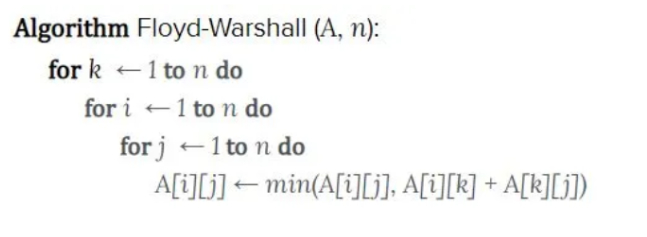
\includegraphics[width=0.8\textwidth]{distancias_cortas_Pseudo1.png}
	\caption{Pseudocódigo de Floyd Warshall.}
	\label{fig:resultado}
\end{figure}

\subsubsection{Código}
\begin{lstlisting}
	import sys
	INF = sys.maxsize
	#Implementacion
	def Floyd_Warshall(graph):
	n = len(graph)
	dist = [[] for i in range(n)]
	for i in range(n):
	for j in range(n):
	dist[i].append(graph[i][j]) #inicializar matriz de distancias
	
	for k in range(n):
	for i in range(n):
	for j in range(n):
	dist[i][j] = min(dist[i][j], dist[i][k] + dist[k][j])
	#Imprimir solucion
	print('Distancia mas corta entre todo par de nodos:')
	for i in range(n):
	for j in range(n):
	if dist[i][j] == INF:
	print("%7s" % ("INF"), end = ' ')
	else:
	print("%7s" % (dist[i][j]), end = ' ')
	print()
	#Grafo
	graph = [ [0, 700, 200, INF, INF, INF],
	[700, 0, 300, 200, INF, 400],
	[200, 300, 0, 700, 600, INF],
	[INF, 200, 700, 0, 300, 100],
	[INF, INF, 600, 300, 0, 500],
	[INF, 400, INF, 100, 500, 0]
	]
	Floyd_Warshall(graph)
	
\end{lstlisting}

\subsubsection{Resultado}
%%%%%%%%%
\begin{figure}[H]
	\centering
	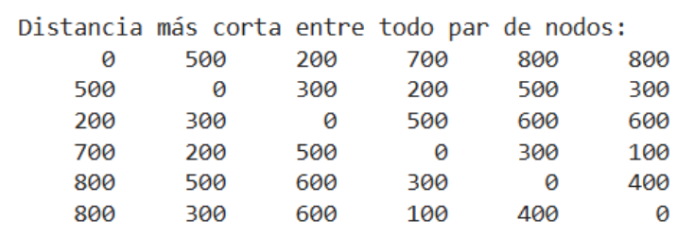
\includegraphics[width=0.8\textwidth]{resultado_distancias_ejem1.png}
	\caption{Resultado de la ejecución del código Python.}
	\label{fig:resultado}
\end{figure}

\subsubsection{Análisis de complejidad}
%%%%%%%%%%%%%%%%%%
\begin{figure}[H]
	\centering
	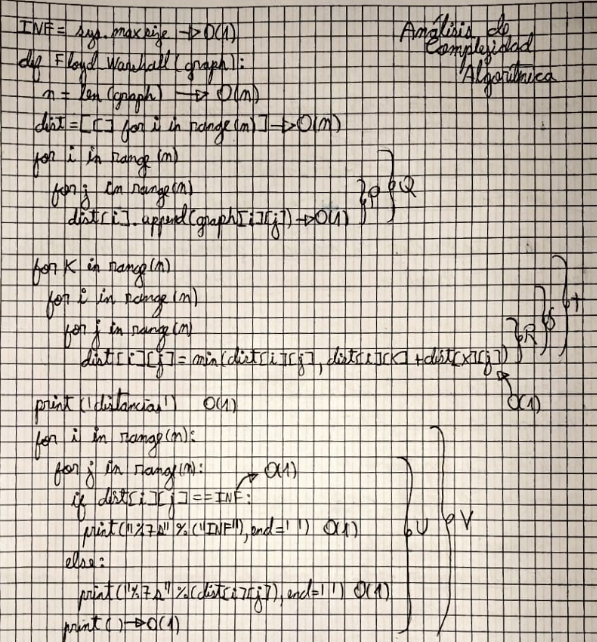
\includegraphics[width=0.8\textwidth]{complejidad_distancia_ejem1_1.png}
	\caption{Analisis del codigo.}
	\label{fig:complejidad1}
\end{figure}
%%%%%%%%%%%%%%%%%%
\begin{figure}[H]
	\centering
	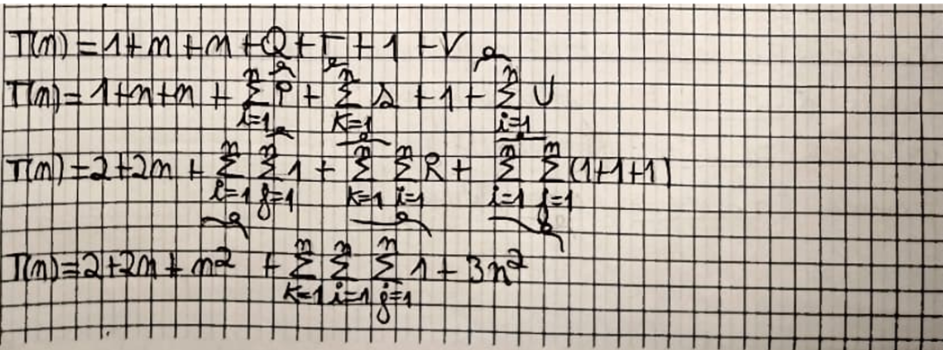
\includegraphics[width=0.8\textwidth]{complejidad_distancia_ejem1_2.png}
	\caption{Analisis del codigo.}
	\label{fig:complejidad1}
\end{figure}
%%%%%%%%%%%%%%%%%%
\begin{figure}[H]
	\centering
	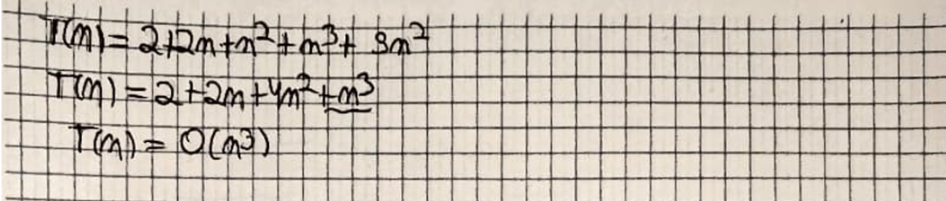
\includegraphics[width=0.8\textwidth]{complejidad_distancia_ejem1_3.png}
	\caption{Analisis del codigo.}
	\label{fig:complejidad1}
\end{figure}


Como es posible apreciar, el uso del algoritmo tiene un costo aproximado de $n^3$, lo cual no representa muy favorable en términos de eficiencia.

\subsection{Ejemplo 2}
\textbf{Algoritmo de Bellman-Ford}

Eres ingeniero de sistemas especializado en redes en una empresa en la que trabajas. Se calculan los tiempos que demoran para comunicarse entre distintos routers. Se te pide por tanto hallar el menor tiempo posible para comunicarte desde el Router Riobamba hacia todos los demás routers. 

%%%%%%%%%
\begin{figure}[H]
	\centering
	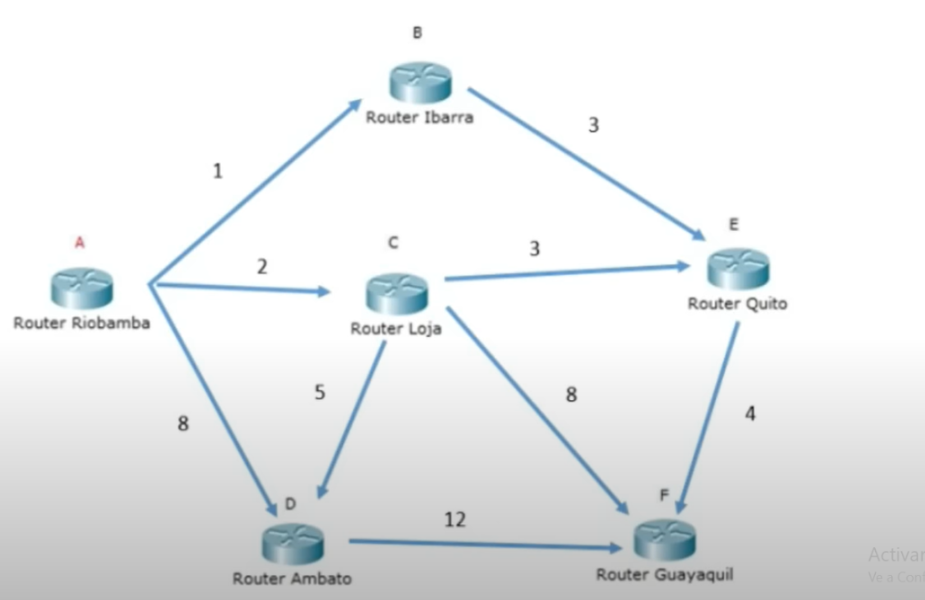
\includegraphics[width=0.8\textwidth]{distancias_cortas_RepresentacionG1_ejem2.png}
	\caption{Representación gráfica del problema.}
	\label{fig:resultado}
\end{figure}


Uno de los algoritmos más utilizados en programación dinámica para este tipo de problemas es el algoritmo de Bellman-Ford, cuyo pseudocódigo es el siguiente:

%%%%%%%%%
\begin{figure}[H]
	\centering
	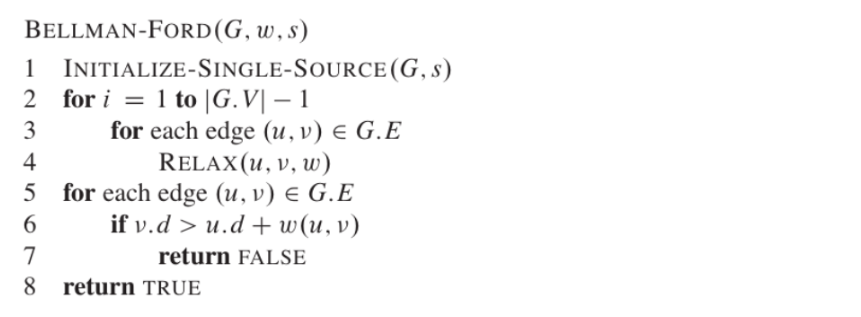
\includegraphics[width=0.8\textwidth]{distancias_cortas_Pseudo2.png}
	\caption{Pseudocódigo de Bellman-Ford.}
	\label{fig:resultado}
\end{figure}

\subsubsection{Código}
\begin{lstlisting}[language=Python]
	#Diccionario de aristas y sus pesos
	w = {
		(0,1) : 1,
		(0,5) : 2,
		(0,4) : 8,
		(1,2) : 3,
		(2,3) : 4,
		(4,3) : 12,
		(5,2) : 3,
		(5,3) : 8,
		(5,4) : 5
	}
	
	#numero de vertices
	n = 6
	
	def relax (u,v,w,d,p):
	if d[v] > d[u] + w[u,v]:
	d[v] = d[u] + w[u,v]
	p[v] = u
	
	def Bellman_Ford(w,n,s):
	
	inf = 1e100
	d = [0 for i in range(n)] ##Es la cota superior del peso del camino mas corto de s a v, se inicializa en infinito
	p = [0 for i in range(n)] ##Es el nodo previo en el camino del peso mas corto de s a v
	
	for vertex in range(n):
	d[vertex] = inf #Asumimos infinito al principio, es decir, es desconocido el limite
	p[vertex] = 'null' #Aun no sabemos el nodo previo de vertex en el camino mas corto
	
	d[s] = 0 #0 porque el peso de s a s es 0
	
	for _ in range (n-1):
	for u,v in w:  #arista (u,v) : peso
	relax(u,v,w,d,p) #actualizacion de las distancias
	
	for (u,v) in w: #detectar ciclos negativos
	if d[v] > d[u] + w[u,v]:
	return False
	
	print("Distancias mas cortas")
	for i in range(n):
	print(i, ": ", d[i])
	
	print("\nNodos previos")
	for i in range(n):
	print(i, ": ", p[i])
	
	return True
	
	Bellman_Ford(w,n,0)
	
\end{lstlisting}

\subsubsection{Resultado}
%%%%%%%%%%
\begin{figure}[H]
	\centering
	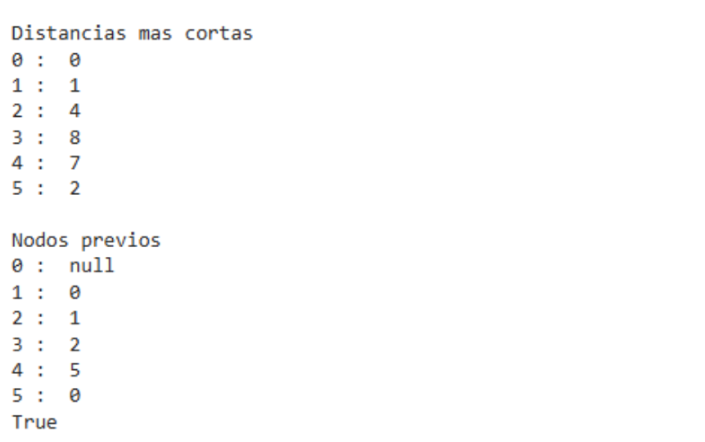
\includegraphics[width=0.8\textwidth]{resultado_distancias_ejem2.png}
	\caption{Resultado de la ejecución del codigo Python.}
	\label{fig:resultado}
\end{figure}

\subsubsection{Análisis de complejidad}
%%%%%%%%%%%%
\begin{figure}[H]
	\centering
	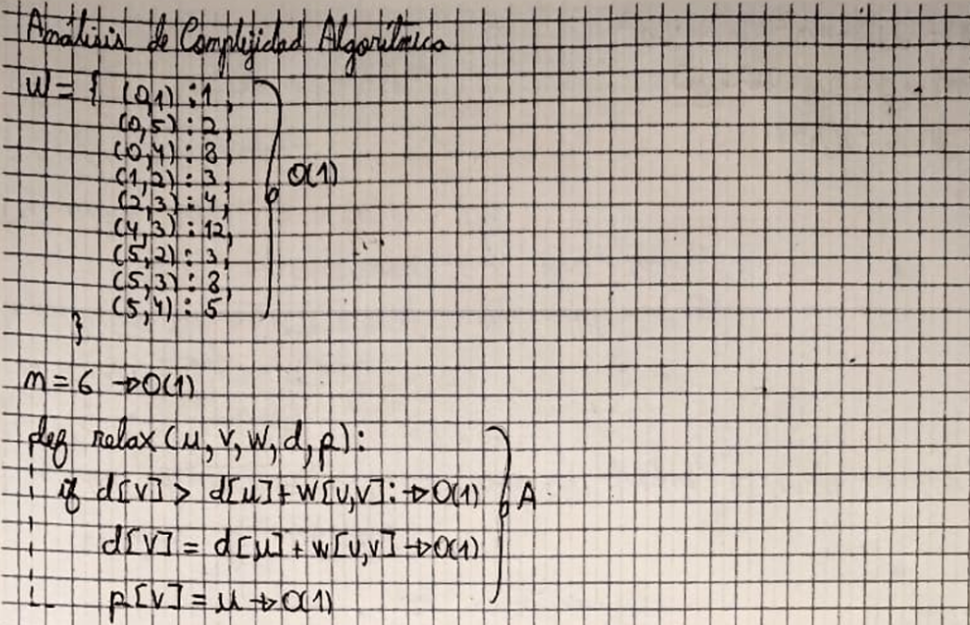
\includegraphics[width=0.8\textwidth]{complejidad_distancia_ejem2_1.png}
	\caption{Analisis del codigo.}
	\label{fig:complejidad1}
\end{figure}

%%%%%%%%%%%%
\begin{figure}[H]
	\centering
	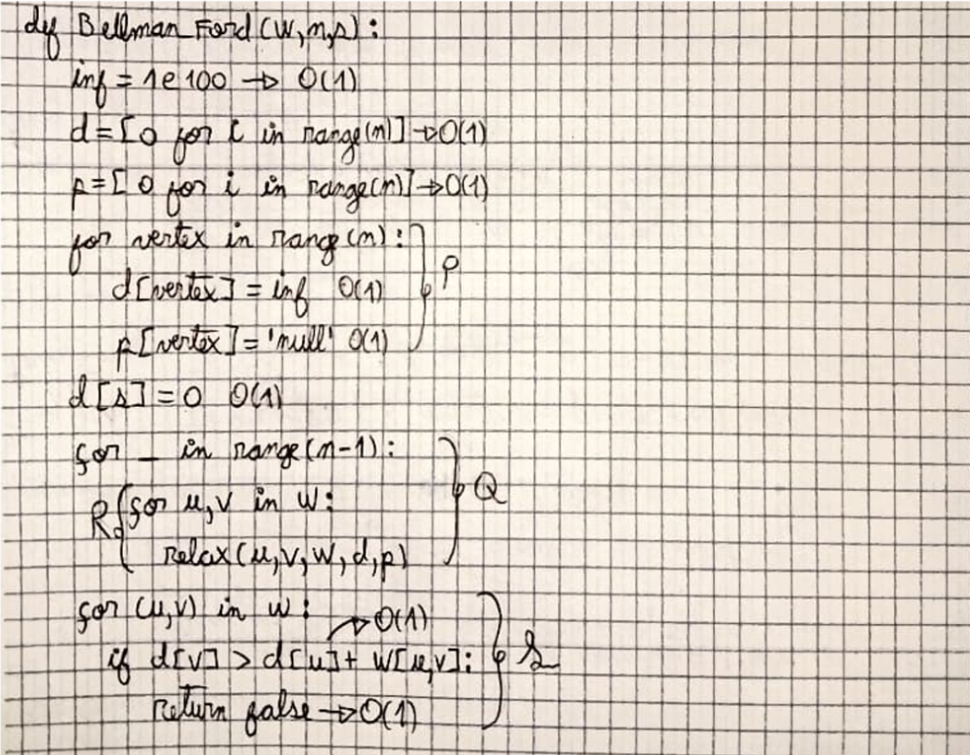
\includegraphics[width=0.8\textwidth]{complejidad_distancia_ejem2_2.png}
	\caption{Analisis del codigo.}
	\label{fig:complejidad1}
\end{figure}
%%%%%%%%%%%%
\begin{figure}[H]
	\centering
	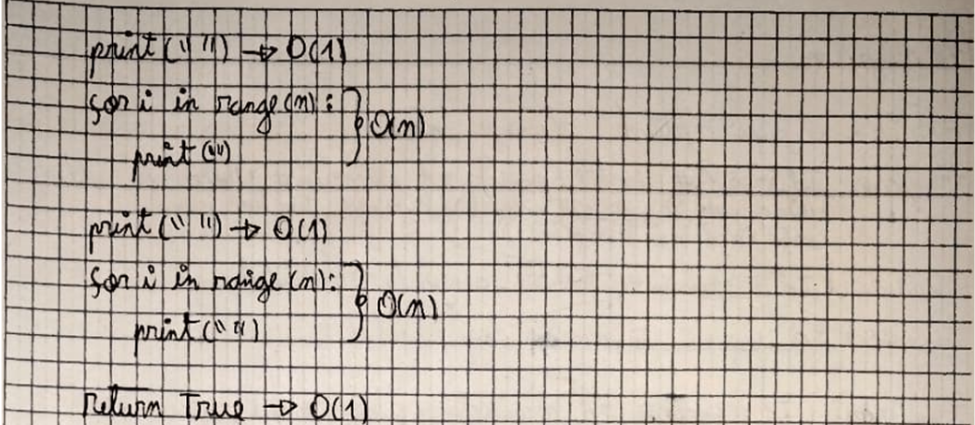
\includegraphics[width=0.8\textwidth]{complejidad_distancia_ejem2_3.png}
	\caption{Analisis del codigo.}
	\label{fig:complejidad1}
\end{figure}
%%%%%%%%%%%%
\begin{figure}[H]
	\centering
	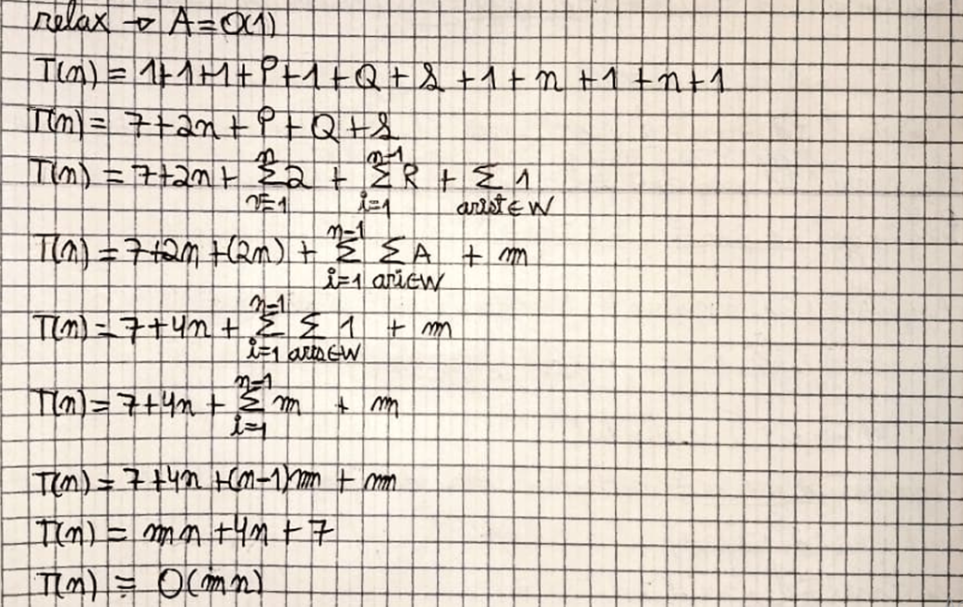
\includegraphics[width=0.8\textwidth]{complejidad_distancia_ejem2_4.png}
	\caption{Analisis del codigo.}
	\label{fig:complejidad1}
\end{figure}
%%%%%%%%%%%%
\begin{figure}[H]
	\centering
	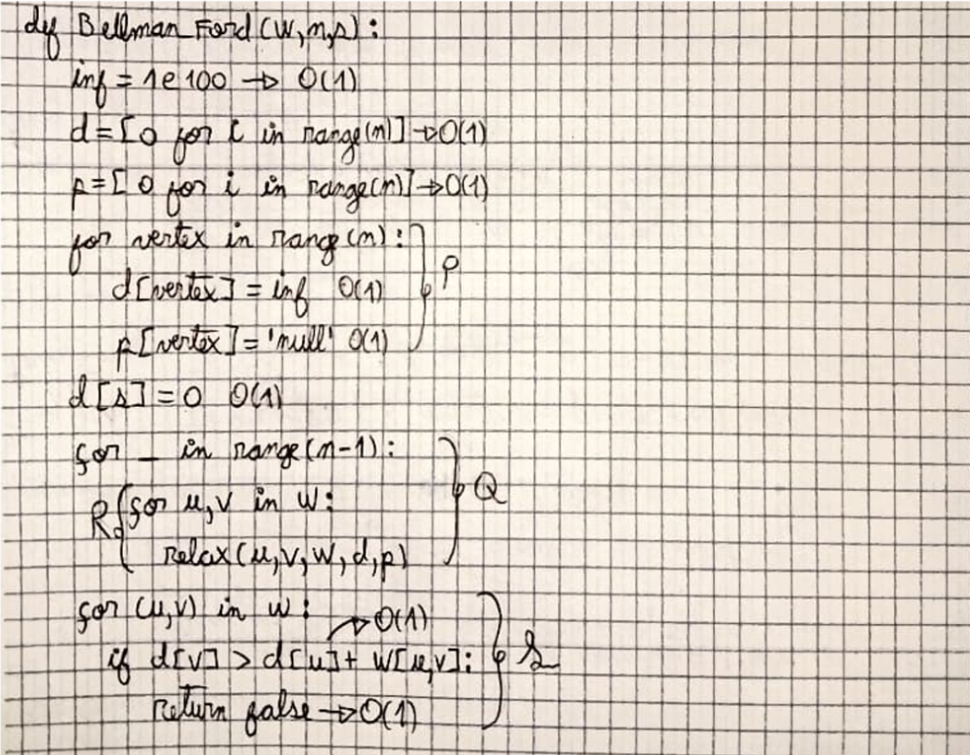
\includegraphics[width=0.8\textwidth]{complejidad_distancia_ejem2_2.png}
	\caption{Analisis del codigo.}
	\label{fig:complejidad1}
\end{figure}

Puede observar que la complejidad es O(m*n), donde m es el numero de aristas y n de nodos. Si m fuera el numero máximo de aristas, la complejidad se define como O($n^3$)
